\chapter{Introduction}
In this chapter, we are going to recapitulate the concept of the
neutrinos $\left(\nu\right)$ and the experimental milestones placed
so far on the path of understandings of this elusive particle. This
chapter also focuses briefly on the India-based Neutrino Observatory
(INO), an effort to dive into the mystery of the neutrinos.

\section{Neutrinos}
The road to the neutrino\cite{roadtoneut}, even though the existence
of it was unknown at the beginning, started with the discovery of
radioactivity by Henri Becquerel in 1896\cite{becquerel1896}, followed
by the identification of the $\beta$-particle by Ernest Rutherford in
1899\cite{rutherford1899}. After that, it took almost 30 years to
establish the fact that the energy spectrum of the electrons emitted
in the $\beta$-decay is continuous, confirmed with the results
published by Charles Drummond Ellis and William Alfred Wooster
in 1927\cite{ellis1927}. In 1929, Meitner and Wilhelm Orthmann
verified the results published by Ellis and William with improved
apparatus\cite{meitner1930}, and then Meitner wrote to Ellis,
``We have verified your results completely. ...... . But I do not understand this result at all.''\cite{lettertoCD}
To explain the continuous energy spectrum of the electron in the
$\beta$-decay, in 1930, Wolfgang Pauli's `desperate way out' was the
suggestion of a very light, neutral and spin $^1/_2$ particle emitted
along with the electron that became known as the neutrino. This did
not contradict with the law of energy, momentum and spin conservation.
Convinced by this, Enrico Fermi incorporated the putative neutrino
into a successful theory of $\beta$-decay. Finally, in 1956, Frederick
Reines and Clyde Cowan delivered the experimental evidence of the
existence of the neutrino (or the Poltergeist, as Reines called it)
by observing the inverse $\beta$-decay, $p+\overline{\nu}_e=e^++n$,
in the high neutrino flux near a reactor\cite{reines1956}.
The discovery of the $\nu_{\mu}$ and $\nu_{\tau}$ were discovered at
the Brookhaven National Accelerator Laboratory in
1962\cite{muonneut1962} and at the DONuT~collaboration in
2000\cite{tauneut2001}, respectively.

The neutrinos are the second most abundant particles in the known
universe, after the photon. They are, till date known to be exist
in three different flavours, verified experimentally in
\mbox{$e^+e^-$-collisions\cite{numberneut}}, named the electron
neutrino $\left(\nu_e\right)$, the muon neutrino
$\left(\nu_{\mu}\right)$ and the tau neutrino $\left(\nu_{\tau}\right)$.

\subsection{Neutrinos in the Standard Model}
The Standard Model (SM) of Particle Physics, formulated by
S. Glashow, S.~Weinberg and A.~Salam, represents the descriptions of the
elementary particles and the fundamental forces in nature
(except gravitational force)\cite{glashow1959, weinberg1967,abdus1968}.
The model is based on
$\text{SU}\left(2\right)\times\text{U}\left(1\right)$ gauge theory
which speculated the existence of the weak neutral
currents\cite{glashow1961}.
The discovery of the neutral current neutrino interactions in 1973
by the Gargamelle experiment at CERN delivered the validation of the
Standard Model\cite{hasert1973,hasert1973_1,hasert1974}, which is
also confirmed by Fermilab independently\cite{benvenuti1974}.
According to the SM, the fundamental building blocks of the observable
universe are made of 12 fermions with spin~$\frac{1}{2}$ (6 leptons and
6 quarks) and their anti-particles. The fermions interact between
each other via 4 gauge bosons with spin~1 which are called as
carriers of interactions. These particles were discovered in various
experiments around the world. The most interesting discovery which
relates directly to the neutrinos is the measurement of the invisible
decay~width of $Z$~boson, performed accurately by the LEP~experiment
at CERN\cite{numberneut}. This measurement has constrained the number
of neutrino flavours to three with satisfactory uncertainty.

According to the Standard Model, all the fermions acquire masses via
the Higgs mechanism. A fermion mass term thus must require a coupling
of the left-handed and the right-handed fields. As the neutrinos have
left-handed helicity and the anti-neutrinos have right-handed
helicity, the SM neutrinos are massless and they favour
leptonic~number conservation. However, the neutrino experiments have
strongly settled the phenomenon of the neutrino flavour mixing
(also called as the neutrino oscillations) which confirms the masses
of the neutrinos to be non-zero. Hence, the understanding of the
mechanism via which the neutrinos gain masses, as well as the neutrino
oscillations are beyond the scope of the Standard Model. Therefore,
the neutrinos are very crucial objects to solve the puzzles of the
new physics lying beyond the Standard Model.


\subsection{Neutrino Interactions}
The neutrinos are weakly interacting particles, which means that they
only interact via $\mathrm{W}^{\pm}$ and $\mathrm{Z}^{0}$ bosons and the
interactions are called charged-current (CC) and neutral-current (NC)
interactions, respectively. As the $\mathrm{W}^{\pm}$ and
$\mathrm{Z}^{0}$ are much heavier members in the family of
intermediating particles, the ``week interactions'' which means that
the probability of interaction is very less.

In CC interactions, the neutrino exchanges charge with a nucleon via
$\mathrm{W}^{\pm}$ and turns into a charged lepton associated with the
neutrino. When a high energetic neutrino interacts with the nucleons,
the gluons inside the nucleons also takes part in the interactions,
which leads to the productions of one or many hadrons, apart from the
charged lepton. Unlike CC interactions, the charged leptons are absent
in the final state in the case of NC interactions. In an experiment,
the presence of the charged leptons in the final state distinguishes
between CC and NC events.

\subsection{Sources of Neutrinos}
The neutrinos are produced at numerous different sources, both
\mbox{man-made} and natural, over a wide-range of energy. The
estimated abundance of neutrinos from different sources can be found
in the Figure~\ref{fig:neutrino_flux}. 
\begin{figure}[h]
  \centering
  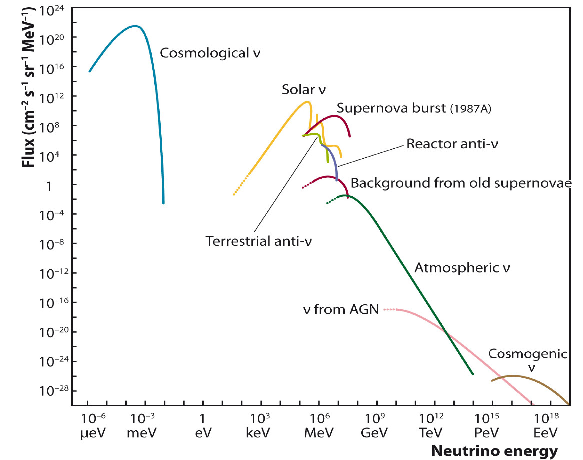
\includegraphics[width=0.8\textwidth]{neutrino_flux.pdf}
  \caption{Predicted flux of neutrinos from different sources
    \cite{neutrinoflux}.}
  \label{fig:neutrino_flux}
\end{figure}

The neutrinos in the energy range of $\mu$eV to meV or the so-called
``relic'' neutrinos are understood to originate at the big-bang
nucleosynthesis \cite{nucleosynthesis}. The neutrinos originated in
the sun\cite{raydavis}, the supernovas, the
earth\cite{kamland,borexino} and the nuclear reactors are of the
energy range of keV to MeV. The neutrinos, being produced by the
interaction of cosmic rays with atmosphere, have energies ranging
from MeV to TeV. The neutrinos produced at supernova remnants,
gamma-ray bursts, active galactic nuclei and from interactions of
ultra-energetic cosmic rays with cosmic microwave background occupy
the higher range of energies.

A few sources being studied in the different experiments are discussed
in the following.

\begin{itemize}
\item \textbf{Solar Neutrinos:} The sun is the most abundant source of
  the electron neutrinos. The Standard Solar Model (SSM)\cite{SSM}
  predicts the production of the neutrinos to be occurring through the
  exothermic nuclear fusion at the core of the sun mainly in two
  processes: (i) proton-proton (pp) cycle and
  (ii) carbon-nitrogen-oxygen (CNO) cycle.
  
  The Solar neutrinos detected at the earth serves as the direct
  telescope to the core of the sun.
  
\item \textbf{Atmospheric Neutrinos:} The atmosphere of the Earth is
  exposed to high energetic primary cosmic rays originating in outer
  space. These cosmic rays consist of mostly protons with a smaller
  fraction of higher \mbox{Z-Nuclei} elements\cite{cosmic1}. The
  energy spectrum of the primary cosmic rays follows a power-law,
  $E^{-\gamma}$ where $\gamma\simeq 2.7$ for sub-TeV energy and 3 for
  beyond. The incoming cosmic rays interact with the constituents
  of the atmosphere producing showers of secondary particles.
  The secondaries are consisting mainly of
  \mbox{pions $\left(\pi^{\pm,0}\right)$} and
  \mbox{kaons $\left(K^{\pm}\right)$}. The neutral pions mainly decay
  via electro-magnetic interactions, $\pi^0 \rightarrow \gamma+\gamma$
  whereas the charged pions decay to muons and neutrinos via
  weak-interactions, $\pi^+ \rightarrow \mu^+ + \nu_{\mu}$ and
  $\pi^- \rightarrow \mu^- + \bar{\nu}_{\mu}$. The resultant muons may
  also decay into electrons and neutrinos,
  $\mu^+ \rightarrow e^+ + \nu_{e} + \bar{\nu}_{\mu}$ and
  $\mu^- \rightarrow e^- + \bar{\nu}_{e} + \nu_{\mu}$. The kaons also
  decay to muons and neutrino and to pions in different branching
  fractions, but this contribution to the atmospheric neutrinos flux
  $\left(\Phi\right)$ is small compared to the pions. The production
  of $\left(\nu_{\tau}\right)$ is negligible in the atmosphere as the
  production needs mesons with heavier quarks.
  
  The ratio, $R$, between $N_{\mu}\left(\propto \Phi\left(\nu_{\mu}\right)+\Phi\left(\bar{\nu}_{\mu}\right)\right)$ and $N_{e}\left( \propto\Phi\left(\nu_{e}\right)+\Phi\left(\bar{\nu}_{e}\right)\right)$ is predicted to be around 2,
  near the surface of the earth. The value of $R$ increases with
  energy as muons with high energy reach the surface of the earth
  before decaying.
  
  The plentiful atmospheric neutrinos, for its wide range of energy
  and for being `cost-free', are very important in the field of
  neutrino research.
  
\item \textbf{Reactor Neutrinos:} The fission reactions of heavy
  nuclei like $U^{235}$, $U^{238}$, $P^{239}$, $P^{241}$, etc. produce
  $\bar{\nu}_{e}$ through the process of $\beta$-decay in the reactor
  cores. As the reactor neutrinos derive their energy from these
  fission reaction, the energy of these $\bar{\nu}_{e}$s are in the
  MeV range, typically within 2-3\,MeV with a significant tail till
  about 8\,MeV.

  The high flux of neutrinos near a reactor provides a brilliant
  experimental scope of studying the properties of neutrinos. So, the
  importance of the reactor neutrinos dates back to the experiment by
  Reines and Cowan which provided the first experimental evidence of
  the existence of the neutrinos.
  
\item \textbf{Accelerator Neutrinos:} Accelerator neutrinos are
  produced at large scale particle accelerators. When a high energy
  proton beam collides with a heavy nuclei target, a bunch of pions
  and kaons are produced. These pions and kaons eventually decay into
  neutrinos, electrons/muons and mesons. There are long shields placed before the
  detector to filter the mesons from the neutrino beam. Mainly,
  $\bar{\nu}_{\mu}$s and $\nu_{\mu}$ are produced at the accelerators,
  but the beam may get contaminated by the production of
  $\bar{\nu}_{e}$ and $\nu_{e}$ from the decay of a certain fraction
  of kaons. By the selection and manipulation of the beam of pions and
  kaons, proper control on neutrino type and energy can be achieved,
  making the accelerator neutrinos one of the vital source for the
  detailed study of neutrino phenomenon.
  
\end{itemize}


\subsection{Neutrino Oscillations}
The concept of neutrino oscillations was first proposed by Bruno
Pontecorvo in 1957\cite{pontecorvo1,pontecorvo2}. The neutrino
oscillation is of great theoretical and experimental interest as it
implies that neutrino has non-zero mass, which leads to modification
of the Standard Model of particle physics. The neutrino oscillations occur due to the mixing of the flavour eigenstates and mass eigenstates of
neutrinos. The visual flavour eigenstates
$\left(\ket{\nu_{\alpha}};\alpha=e,\mu,\tau\right)$ can be expressed as
a linear combination of the mass eigenstates
$\left(\ket{\nu_{j}};j=1,2,3\right)$ as shown in the following equation.
\begin{equation}
  \ket{\nu_{\alpha}}=\sum_{j}U_{\alpha j}\ket{\nu_{j}} \label{eq:tzero}
\end{equation}
The unitary mixing matrix, $U$, called the PMNS matrix, is named after
Pontecorvo, Maki, Nakagawa and Sakata. The mixing of three flavours of
neutrinos can be defined with 3 mixing angles and 6 phases. Five of
the phases can be absorbed into fermion fields in Kobayashi-Maskawa
mechanism\cite{kobayashimaskawa}. Only one phase has an effect which
leads to CP~Violation in neutrino oscillations. The mixing matrix with
three mixing angles ($\theta_{12}$, $\theta_{23}$ and $\theta_{13}$) and
one phase ($\delta_{\mathrm{CP}}$) is represented in the following,
\begin{equation}
  U_{\mathrm{PMNS}} =
  \underbrace{\begin{bmatrix}
      1 & 0 & 0 \\
      0 & c_{23} & s_{23} \\
      0 & -s_{23} & c_{23}
    \end{bmatrix}
  }_{\text{Atmospheric }\left(\theta_{23}\sim 48^{\circ}\right)}
  \underbrace{\begin{bmatrix}
      c_{13} & 0 & s_{13}e^{-\mathrm{i}\delta_{\mathrm{CP}}} \\
      0 & 1 & 0 \\
      -s_{13}e^{\mathrm{i}\delta_{\mathrm{CP}}} & 0 & c_{13}
    \end{bmatrix}
  }_{\text{Reactor }\left(\theta_{13}\sim 8.5^{\circ}\right)}
  \underbrace{\begin{bmatrix}
      c_{12} & s_{12} & 0 \\
      -s_{12} & c_{12} & 0 \\
      0 & 0 & 1
    \end{bmatrix}
  }_{\text{Solar }\left(\theta_{12}\sim 34^{\circ}\right)}
   \label{eq:pmns}
\end{equation}
where, $c_{jk}=\cos\theta_{jk}$ and $s_{jk}=\sin\theta_{jk}$.

The time evolution of the states in equation~\ref{eq:tzero} is given
by the following equation,
\begin{equation}
  \ket{\nu_{\alpha}\left(t\right)}=\sum_{j}U_{\alpha j}e^{-\mathrm{i}E_{j}t}\ket{\nu_{j}} \label{eq:ttime}
\end{equation}
where, $E_{j}\left(=\sqrt{p_{j}^{2}+m_{j}^{2}}\right)$ is the energy
eigen values corresponds to the vacuum propagation Hamiltonian
$\left(H_0\right)$.

The probability of oscillating from the flavour state $\nu_\alpha$ to
the state $\nu_\beta$ is given in the following equation,
\begin{equation}
  P_{\nu_\alpha\rightarrow\nu_\beta}\left(t\right) = \left|\braket{\nu_\beta|\nu_\alpha\left(t\right)}\right|^2 = \sum_{j,k}U_{\alpha j}U^{*}_{\beta j}U^{*}_{\alpha k}U_{\beta k}e^{-\mathrm{i}\left(E_{j}-E_{k}\right)t}.
  \label{eq:oscprob}
\end{equation}
If $\nu_\alpha=\nu_\beta$, then $P$ is called the `survival probability',
and `oscillation probability' if otherwise.

The equations~\ref{eq:oscprob} also can be expressed in the following
form,
\begin{align}
  P_{\nu_\alpha\rightarrow\nu_\beta}\left(L\right) = \delta_{\alpha\beta} & -4\sum_{j>k}\Re\left[U_{\alpha j}U^{*}_{\beta j}U^{*}_{\alpha k}U_{\beta k}\right]\sin^2\left(\frac{\Delta m^2_{jk}L}{4E}\right) \nonumber\\
  & +2\sum_{j>k}\Im\left[U_{\alpha j}U^{*}_{\beta j}U^{*}_{\alpha k}U_{\beta k}\right]\sin\left(\frac{\Delta m^2_{jk}L}{2E}\right)
  \label{eq:lprob}
\end{align}
where, $\Delta m^2_{jk}=m^2_{j}-m^2_{k}$.

The oscillation probability for the anti-neutrinos thus given by
\begin{align}
  P_{\bar{\nu}_\alpha\rightarrow\bar{\nu}_\beta}\left(L\right) = \delta_{\alpha\beta} & -4\sum_{j>k}\Re\left[U^{*}_{\alpha j}U_{\beta j}U_{\alpha k}U^{*}_{\beta k}\right]\sin^2\left(\frac{\Delta m^2_{jk}L}{4E}\right) \nonumber\\
  & +2\sum_{j>k}\Im\left[U^{*}_{\alpha j}U_{\beta j}U_{\alpha k}U^{*}_{\beta k}\right]\sin\left(\frac{\Delta m^2_{jk}L}{2E}\right).
  \label{eq:laprob}
\end{align}

The equation \ref{eq:lprob} and \ref{eq:laprob} show that the neutrino
oscillations can only exist if the masses of neutrinos are
non-zero. It is also seen that the real parts of the equation
\ref{eq:lprob} and \ref{eq:laprob} are CP invariant. So, the CP
asymmetry can be interpret as,
\begin{equation}  P_{\nu_\alpha\rightarrow\nu_\beta}\left(L\right)-P_{\bar{\nu}_\alpha\rightarrow\bar{\nu}_\beta}\left(L\right) = 4\sum_{j>k}\Im\left[U_{\alpha j}U^{*}_{\beta j}U^{*}_{\alpha k}U_{\beta k}\right]\sin\left(\frac{\Delta m^2_{jk}L}{2E}\right).
  \label{eq:cpass}
\end{equation}

It is to be noted that the equation \ref{eq:lprob} and \ref{eq:laprob}
do not provide any resolution about the sign of the $\Delta m_{jk}^{2}$s
or the absolute values of $m_{j}$s.

\subsubsection{$\bullet$ Neutrino Oscillations in Matter}

When neutrinos pass through matter, then probabilities of oscillations
can also be altered due to the`matter-effect'. The neutrinos face
coherent forward scattering with the electrons, protons and neutrons
present in the matter \cite{mattereffect}. The potential arising due to
this effect modifies the vacuum propagation Hamiltonian
$\left(H_{0}\right)$, effecting the mixing of neutrinos.

This phenomenon of altering neutrino flavour during propagation in the
matter was introduced by Mikhaev, Smirnov and Wolfenstein
(MSW)\cite{msw1}. The $\nu_{e}$s have both CC with electrons and NC elastic 
scattering interactions with electrons, protons, neutrons present in matter, 
but the $\nu_{\mu}$s and
$\nu_{\tau}$s have only NC interactions with matters. The potential
$V_{\textrm{NC}}$ is experienced by all three flavours. The additional
CC interactions account for an extra potential $V_{\textrm{CC}}$. Hence, the
matter Hamiltonian is given as,
\begin{equation}
  H_{\mathrm{m}} = H_{0}+V_{\mathrm{m}}
\end{equation}
where, $V_{\mathrm{m}}$ is represented as,
\begin{equation}
  V_{\mathrm{m}} =
  \begin{bmatrix}
    V_{\textrm{CC}} + V_{\textrm{NC}} & 0 & 0 \\
    0 & V_{\textrm{NC}} & 0 \\
    0 & 0 & V_{\textrm{NC}}
  \end{bmatrix}.
\end{equation}
where, $V_{\textrm{CC}} = \sqrt{2}G_{\mathrm{F}}n_{e}$ and
$V_{\textrm{NC}} = -\frac{1}{\sqrt{2}}G_{\mathrm{F}}n_{n}$ are called the effective
potentials. Here, $n_{e}$ and $n_{n}$ are the number densities of electrons and
neutrons, respectively and $G_{\mathrm{F}}$ is the Fermi coupling
constant.
The normalised eigen vectors of the diagonalised matter Hamiltonian form the
modified mixing matrix. Thus, the effective mass-squared differences and mixing
angles can be computed in matter. If two flavour mixing is considered, the
matter affected mass-squared difference $\left(\Delta m^{2}_{m}\right)$ and
mixing angle $\left(\theta_{m}\right)$ are given by,
\begin{equation}
  \tan 2\theta_{m}=\frac{\Delta m^{2}\sin 2\theta}{\Delta m^{2}\cos 2\theta -A} \quad\text{and}\quad \Delta m^{2}_{m} = \sqrt{\left(\Delta m^{2}\cos 2\theta -A\right)^{2} + \left(\Delta m^{2}\sin 2\theta\right)^{2}} \label{eq:mattermass}
\end{equation}
where, $A=2\sqrt{2}G_{\mathrm{F}}n_{e}E$ for neutrinos and
$A=-2\sqrt{2}G_{\mathrm{F}}n_{e}E$ for anti-neutrinos. Here, some points are to
be noted.
\begin{itemize}\itemsep -4pt
\item Assumption of $n_{e}\rightarrow 0$ in the equation~\ref{eq:mattermass}
  makes the matter affected mass-squared difference and mixing angle the same
  as those are in the vacuum. This means that the values of the mass-squared
  differences and the mixing angles from vacuum remain unchanged in matter.
\item If $n_{e}\rightarrow\infty$ and $\theta\neq 0$, then
  $\theta_{m}\rightarrow\frac{\pi}{2}$. Hence, even if the vacuum mixing angle
  is very small, maximum mixing of neutrino can be observed in matter.
\item When $A = \Delta m^{2}\cos 2\theta$, then the value of $\theta_{m}$ goes
  to $\frac{\pi}{4}$. This phenomenon is called the MSW~resonance effect.
  The neutrinos going through MSW~resonance have the maximal probability of
  changing its flavour. Depending on whether the value of $\Delta m^{2}$ is
  positive or negative, the resonance occurs for the neutrinos or
  anti-neutrinos, respectively.
\end{itemize}
For three flavours mixing or in the case of non-uniform matter density, the oscillation probabilities are required to be calculated numerically.

The survival probability of solar neutrinos, predicted by MSW~theory and confirmed by several experiments\cite{homestake,gallex,sage,superk,sno,kamland}, requires $\Delta m_{21}^{2}$ to be positive, but the sign of $\Delta m_{32}^{2}$ is still unknown. Thus, two different mass-ordering of the neutrinos are possible: (i) $m_{1}<m_{2}<m_{3}$ called as normal~hierarchy (NH) or normal~ordering (NO) and (ii) $m_{3}<m_{1}<m_{2}$ called inverted~hierarchy (IH) or inverted~ordering (IO).


\subsection{Status of Neutrino Oscillations Parameters}
Many experiments worldwide are in constant effort to improve the
best-fit values of the oscillation parameters. The detailed summary
on the oscillation parameters from the global analysis, updated in
2018, can be found in \cite{neutrinostatus}.

The best-fit values of mixing angles are reported as
$\theta_{12}\sim 34^{\circ}$, $\theta_{23}\sim 48^{\circ}$ and
$\theta_{13}\sim 8.5^{\circ}$ along with the mass-squared differences as
$\Delta m^2_{21}\sim 7.5\times 10^{-5}$\,eV$^{2}$,
$\left|\Delta m^2_{31}\right|\sim 2.5\times 10^{-3}$\,eV$^{2}$.\footnote{Please refer to \cite{neutrinostatus} for the current accepted/updated values of the oscillations parameters with the uncertainties.}
The global analysis have found preference for the value of
$\delta_{\mathrm{CP}}$ in the range between $\pi$ and $2\pi$ at more than
$4\sigma$\cite{neutrinostatus}. The current combined analysis prefers
the octant of $\theta_{23}$ to be the second octant, slightly. Most
interestingly for the first time, the global analysis favours the
normal mass ordering over the inverted one at
$3.4\sigma$\cite{neutrinostatus}.

\subsection{Study of the Atmospheric Neutrinos}
Unlike the reactor-based or accelerator-based neutrino experiments,
the atmospheric neutrino detectors are not limited by the fixed-length
$\left(L\right)$ between the detector and source of neutrinos or by
the narrow range of energy $\left(E\right)$. The detectors for
atmospheric neutrinos are usually built under a depth of the earth's
surface to reduce the cosmic muon background. Thus, the distances
travelled by the neutrinos detected in these detectors vary up-to a
distance equivalent to the earth's diameter
$\left(\sim 12000\text{\,km}\right)$ after being produced in the
atmosphere. Moreover, the energy of the atmospheric neutrinos ranges
from hundreds of MeV to TeV. This qualifies the atmospheric neutrino
detectors to study the neutrinos over widely varying baselines
$\left(^{L}/_{R}\right)$.

There have been two types of detector commissioned in atmospheric
neutrino research, till date; water Cherencov detectors and tracking
calorimeter detectors. The INO-ICAL which belongs to the latter type
is discussed in the next section.

\section{The India-based Neutrino Observatory}
The India-based Neutrino Observatory (INO)\cite{inowhite,inoreport}
is a multi-institutional effort to build an underground laboratory to
study atmospheric neutrinos. The proposed observatory will be located
at West Bodi Hills near Pottipuram Village (9$^\circ$57$'$36$''$\,N,
77$^\circ$16$'$24$''$\,E). The detectors will be housed inside several
caverns with an overburden of $\sim$1\,km rock in order to reduce the
background due to cosmic muons produced along with the neutrinos. One
big cavern will encase the Iron CALorimeter (ICAL) along with several
small caverns facilitating a few daughter experiments.

\subsection{Physics Aspects of INO-ICAL}
The ICAL is primarily designed to observe the charged-current
interactions of the $\nu_{\mu}/\bar{\nu}_{\mu}$s with the ability to
distinguish between the charged leptons, mainly $\mu^{+}$ and $\mu^{-}$,
which are being produced in the interactions. This ability gives ICAL
advantage to study matter-effect in details and hence to determine the
neutrino mass ordering. The baselines of ICAL vary up-to
$\sim 10000$\,km with wide range of energy from hundreds of MeV to
TeV, which also makes ICAL suited for precise measurement of
atmospheric oscillation parameters. %  and the CP-phase $\left(\delta_{cp}\right)$.

\subsection{The ICAL Detector}
The ICAL detector, with a target medium of $\sim 50$\,kton iron, is a
magnetised calorimeter designed to detect the charge and momentum of
the leptons, mainly $\mu^{\pm}$, produced by the CC interactions by
$\nu_{\mu}/\bar{\nu}_{\mu}$ with detector volume. The Resistive Plate
Chamber (RPC) has been chosen as the active detector element for the
ICAL detector, interspersed with 5.6\,cm thick iron plates.
Approximately 30000 RPC gaps of dimension 2\,m\,$\times$\,2\,m will
be placed in between the 151 layers of iron plates. The iron plates
will be magnetised up-to about 1.5\,Tesla. The dimensions of the
detector are 48\,m, 16\,m and 15\,m. A schematics of ICAL is shown in
the Figure~\ref{fig:icalsk}. 
\begin{figure}[h]
  \centering
  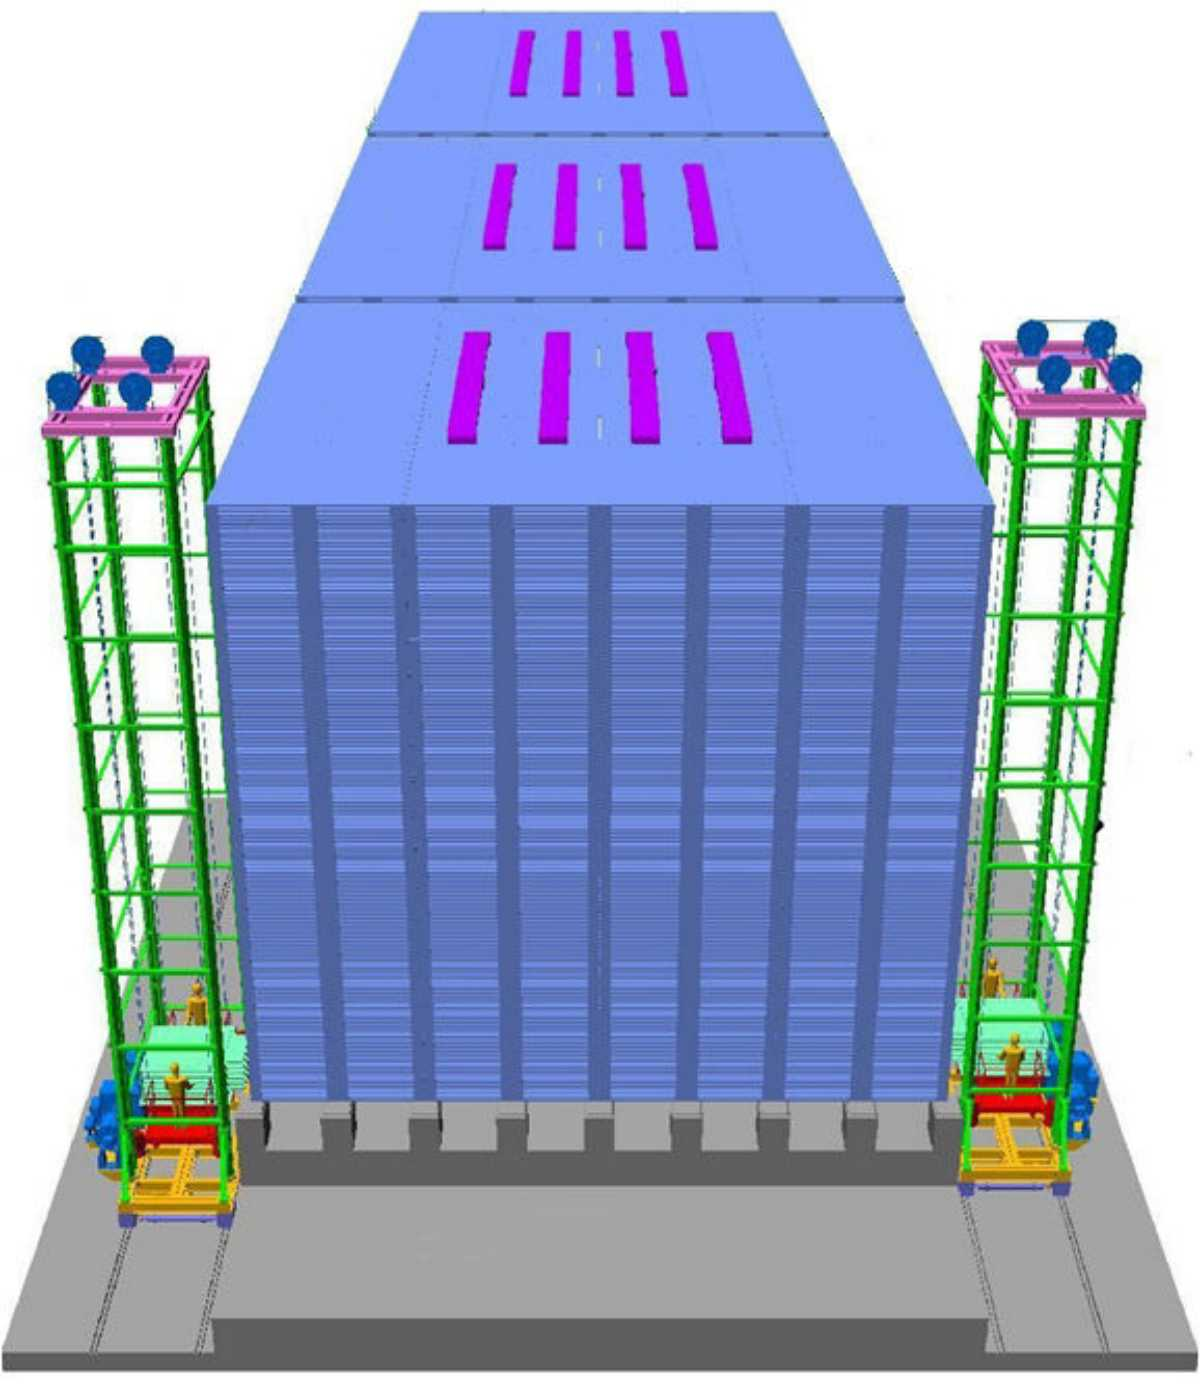
\includegraphics[width=0.5\textwidth]{ical.png}
  \caption{A Schematics of the ICAL detector\cite{inoreport}.}
  \label{fig:icalsk}
\end{figure}
A few important constituents of the ICAL detector are discussed below.

\subsubsection*{$\bullet$ The Resistive Plate Chamber}
The RPC is basically a gaseous based parallel-plate
detector\cite{rpc_p2}. The basic components of RPC are shown in the
Figure~\ref{fig:rpc}. 
\begin{figure}[h]
  \centering
  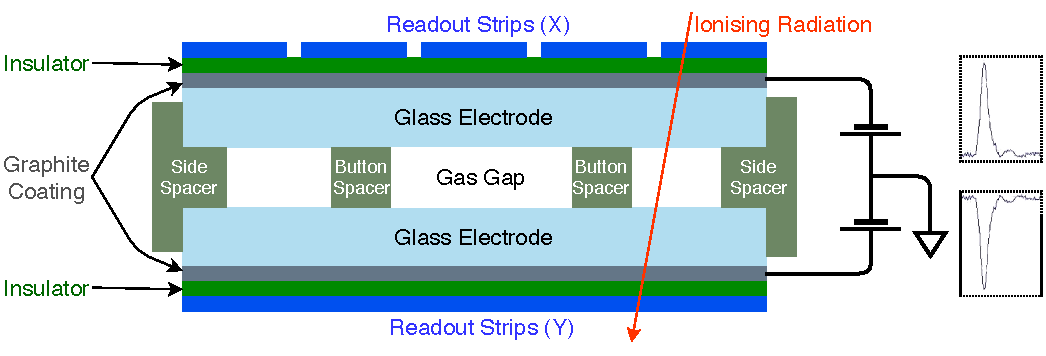
\includegraphics[width=0.6\textwidth]{basic_rpc.pdf}
  \caption{Schematic of a Resistive Plate Chamber.}
  \label{fig:rpc}
\end{figure}
The RPC is constructed using two parallel plates of glass having a
bulk resistivity of the order of $10^{10}$-$10^{12}$\,$\Omega$\,cm with
a gas gap of 2\,mm. Uniform spacing between two glass plates is
maintained using button spacers. Ideally, the whole chamber has to be
leakproof. The outer surfaces of the glass plates are made conductive
using graphite coating to form the electrodes where high voltages can
be applied. The signal is readout by copper pickup panels on both
sides of the RPC. In ICAL detector, the RPCs are going to be operated
in avalanche mode with a gas mixture of R134a\,(95.2\%),
iso-C$_4$H$_{10}$\,(4.5\%) and SF$_6$\,(0.3\%). R134a gas acts as a
target for the ionising particles passing through the gas gap. The
iso-C$_4$H$_{10}$ absorbs the photons emitted in the recombination
processes limiting the formation of secondary avalanches. SF$_6$,
being an electronegative gas, localises the signal in a small area to
have better position resolution.

During the active operation of the ICAL detector, more than
200,000\,litres of the gas mixtures will be circulating inside the
30,000 RPCs. To achieve this, a closed-loop gas circulation system
(CLS) is designed whose main purpose is to recirculate the gas
mixture, minimising wastage of gas which reduces the operational cost.

The RPCs are good charged particle detector with detection efficiency
greater than 95\,\%. Descent detection efficiency along with the time
resolution of $\sim 1$\,ns makes the RPC an excellent component of a
tracker-type detector. Also being comparatively cheaper and
low-maintenance than other detectors used in this field, it is
advantageous to deploy RPCs in a large scale experiment.

\subsubsection*{$\bullet$ The ICAL Magnet}
The iron layers in ICAL serves a dual purpose; as the target for the
neutrinos and to carry the solenoidal magnetic field in the
detector\cite{icalmagnet}. The iron carries a magnetic field up to
1.5\,Tesla. The particles produced by the interactions of the
neutrinos with iron layers propagate in a curved path through the
detector. The curvature of the propagation delivers information about
the charge and momentum of the propagated particle.

The ICAL is divided into three modules as shown in the
Figure~\ref{fig:magnet}(a). 
\begin{figure}[h]
  \centering
  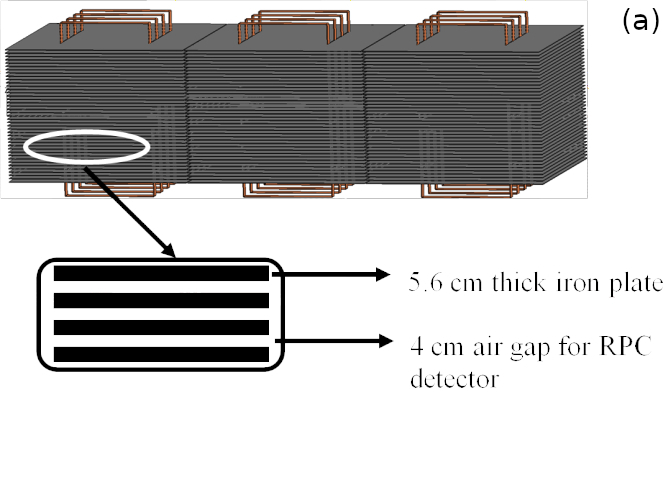
\includegraphics[width=0.48\textwidth]{icalmagnet.jpg}
  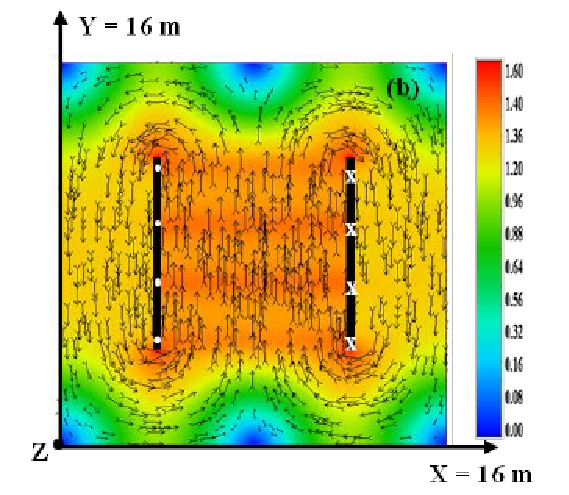
\includegraphics[width=0.48\textwidth]{icalfield.pdf}
  \caption{(a) A Schematics of the ICAL Magnet and (b) Horizontal Projection of the Magnetic field\cite{icalmagnet}.}
  \label{fig:magnet}
\end{figure}
Each of the modules will have two vertical slots cut into the module
to accommodate the winding of the current-carrying copper coils. The
style of the winding makes each of the modules the
`shell-type'\cite{transformer} magnets, thus making the magnetic field
toroidal. The horizontal projection of the magnetic field is shown in
the Figure~\ref{fig:magnet}(b).

\section{Prototype Detector}
As the part of the ICAL R\&D program, several prototype detector
stacks have been built to study the long term stability and
performance of the glass RPC detectors using cosmic muons. The design,
fabrication and characterisation of large-size glass RPCs have already
been examined and reported\cite{largerpc}. One of the stacks was built
at the IICHEP transit campus in Madurai which is shown in the
Figure~\ref{fig:ablock}. This setup is also used as the test-bench
for the data acquisition system (DAQ) schemes which are going to be
used in ICAL detector.
\begin{figure}[h]
  \centering
  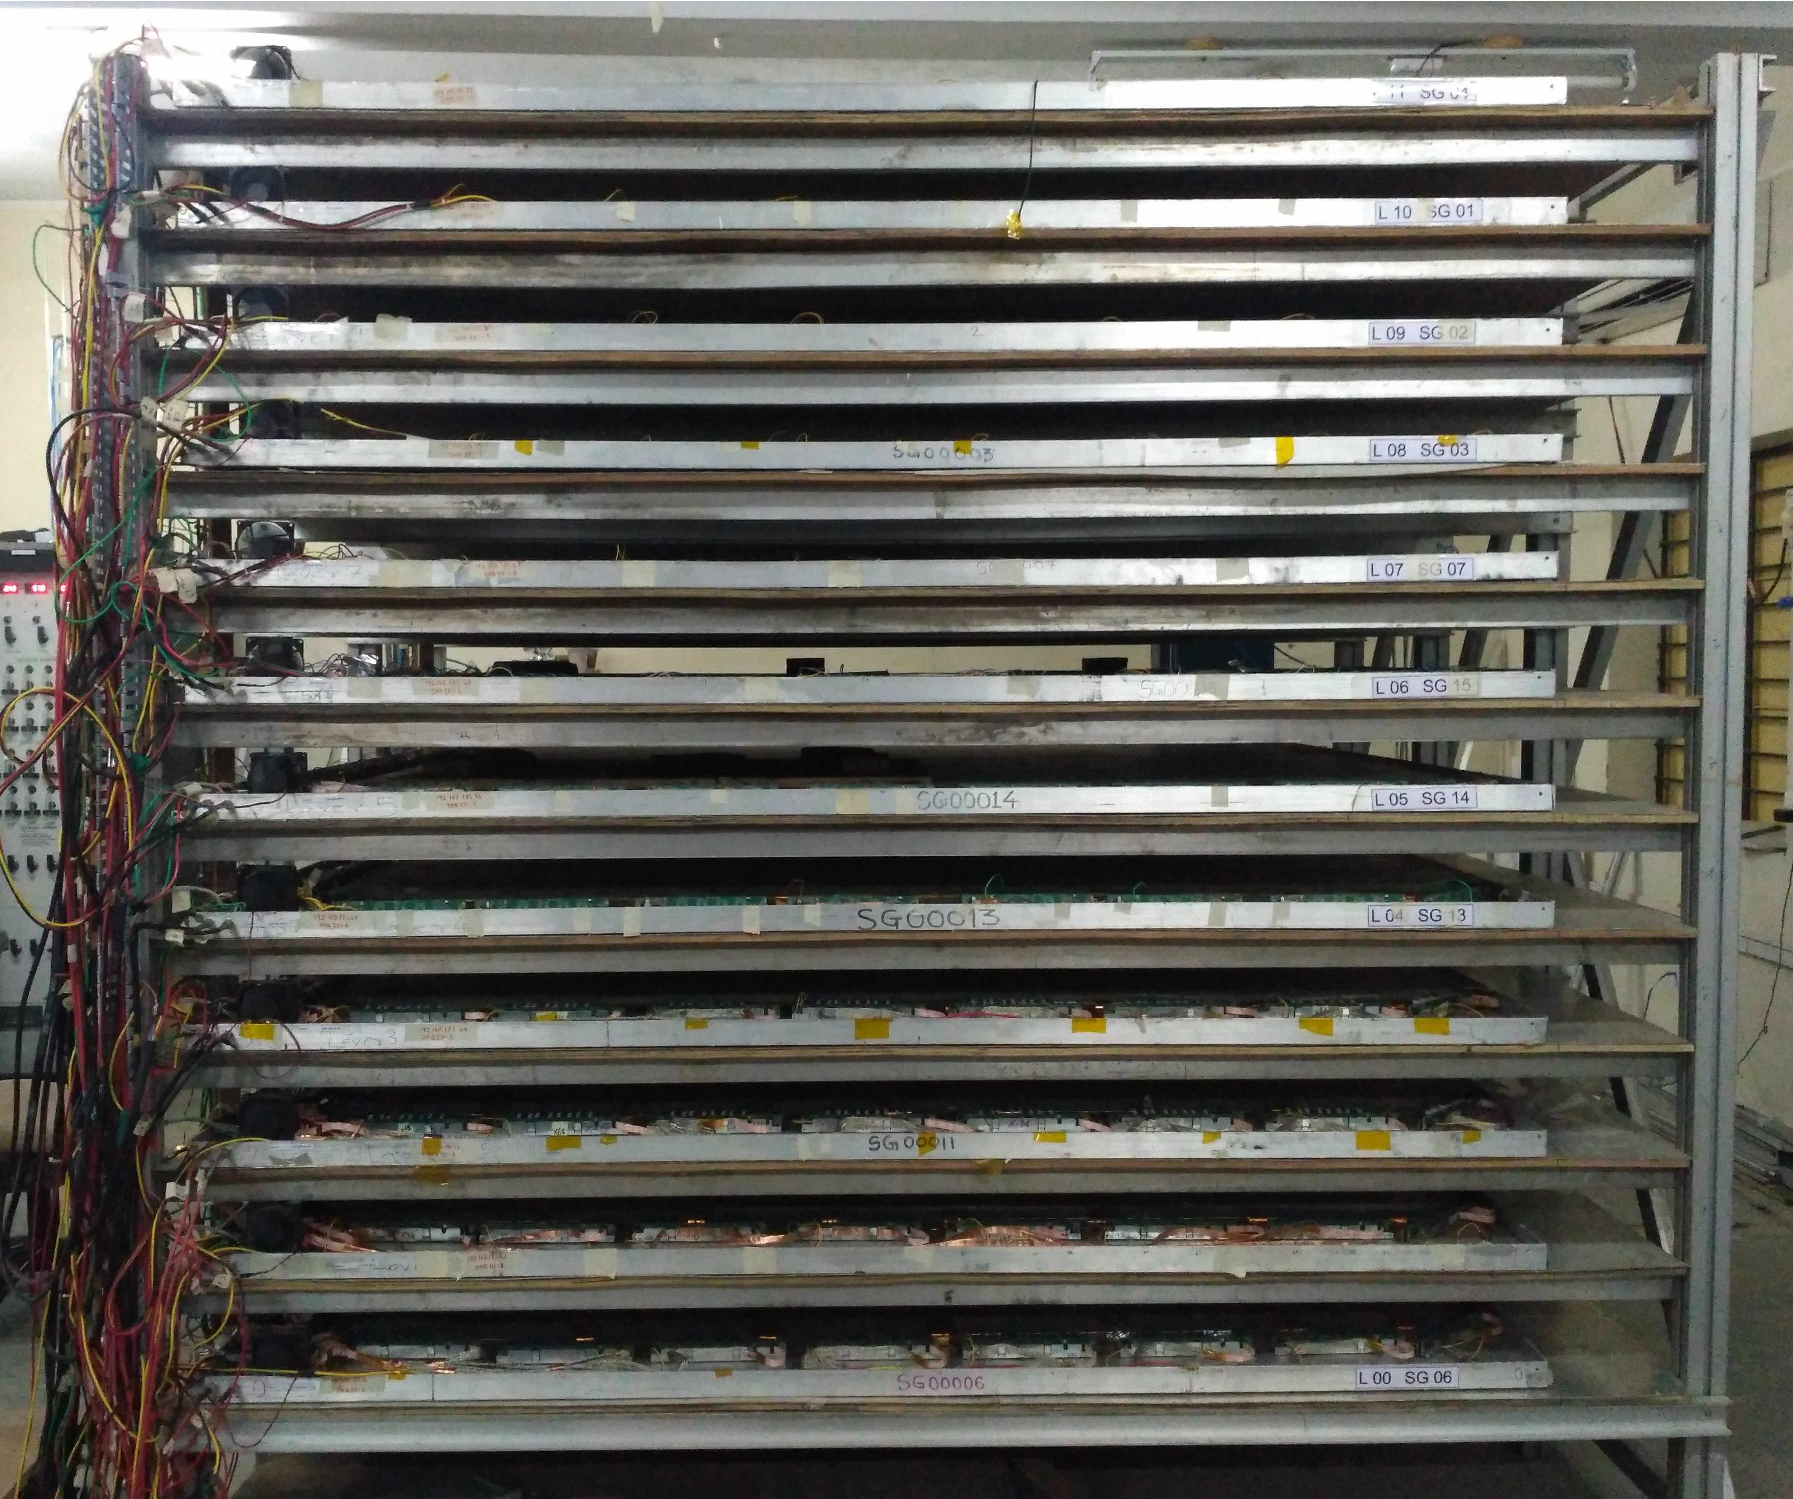
\includegraphics[width=0.85\textwidth]{ABlockStackiDAQ.pdf}
  \caption{Detector Stack with 12 Layers of 2\,m\,$\times$\,2\,m RPCs.}
  \label{fig:ablock}
\end{figure}
The stack is made of 12 layers of 2\,m\,$\times$\,2\,m RPCs with an
inter-layer gap of 16\,cm.

The detector stack is used intensively to study various properties of
the RPCs like strip multiplicities, detector efficiency, detector
noise rate, position resolution, time resolution, etc. The stack also
allows us to study the cosmic ray muons near the equator of the earth.
The data of the cosmic muons collected using these detectors analysed
to study a few important aspects of cosmic rays, i.e. the flux of
the cosmic ray muons at Madurai\cite{pethu1}, magnetic rigidity~cutoff
for the primary cosmic rays at Madurai, particle multiplicity of
secondary cosmic rays at the surface, etc. All of the knowledge gained
by studying the data obtained using this detector stack is used as the
input parameters for the most realistic Monte-Carlo simulations of the
ICAL detector.

\section{miniICAL}
Various tests to study the performance of the magnet assembly is also
performed. To study the magnetic field in the detector and the
performance of the electronics in the presence of magnetic
fringe-field, a detector of the size of $\sim 1/600$ times of ICAL,
named miniICAL, is built at IICHEP transit campus in Madurai. The
detector is consists of 11 layers of soft~iron plates of thickness
5.6\,cm with an interlayer gap of 4.5\,cm. The detector is magnetised
using two copper coils with 18 turns each up-to 1.5\,T. The RPCs are
placed in the interlayer gaps.

The magnetic field profile inside the iron plates is simulated using
2D~Simulation. To validate the result from the simulation, the actual
measurement of the magnetic field is carried out at several strategic
locations of the detector using the help of pick-up coils and
hall~probes. The atmospheric muon data is recorded in miniICAL and
analysed in order to study various detector components. The
performance of the RPCs and the supporting electronics are assessed
under the influence of the magnetic field.

The atmospheric muons passing through the detector leave tracks in the
RPC layers. In the presence of the magnetic field, the muons follow
curved trajectories. The suitable reconstruction algorithm is
developed to extract the momentum and directional information of the
muons from each event. The charge-dependent momentum information of
the muons is computed from this and compared with simulation. This
current measurement along with the existing phenomenological models
can be used
to improve the estimation of neutrino flux at the INO~Site.

\section{Chapter Summary}
The chapter starts with the brief history of the neutrinos followed
by the status of the neutrino oscillations in the global picture. The
INO project is then discussed along with its aim to contribute vital
physics towards the understanding of neutrinos. A brief discussion is
followed afterwards on the RPCs which are being considered as the
sensitive detector in the ICAL detector. The construction and the physics
potential of the ICAL detector is then discussed. Simultaneously, the
scope of the present thesis along with the prototype detectors are
highlighted.
